\label{subart:tmm}
Metoda macierzy przejścia  (ang. transfer matrix method - TMM )~\cite{teich1991fundamentalsTMM} jest używana w~optyce do analizy propagacji fal elektromagnetycznych przez ośrodki warstwowe. Podobne metody w~odniesieniu do ośrodków warstwowych wykorzystywane są w~mechanice kwantowej, akustyce czy sejsmologii. Metoda macierzy przejścia może służyć do wyznaczania współczynników transmisji i~odbicia.

Macierz przejścia dowolnego liniowego i niezmienniczego ze względu na przesunięcia układu optycznego wiąże ze sobą amplitudy pól padających i~wychodzących z układu lub jego fragmentu \cite{markos2008wave,teich1991fundamentalsTMM}:
\begin{equation}
\begin{bmatrix}
U_i \\ 
U_r
\end{bmatrix}
= M 
\begin{bmatrix}
U_t \\
U_b
\end{bmatrix},
\label{eq:tmm}
\end{equation}
gdzie $M$ jest macierzą przejścia warstwowego układu, $U$ jest dowolną wybraną składową pola elektrycznego lub magnetycznego, odpowiednio $U_i$ - padającą, $U_r$ - odbitą, $U_t$ - przechodzącą przez układ oraz $U_b$ padającą  z~przeciwnej strony\footnote{Metodę macierzy przejścia można również zastosować do analizy pola padającego w~postaci dwuwymiarowego rozkładu. W~takim przypadku $U_x$ są wektorami a $M$ tensorem trzeciego rzędu.}. Graficznie sytuację opisywaną powyższym równaniem przedstawia schemat na rysunku~\ref{fig:tmm-simple}.

\begin{SCfigure}
	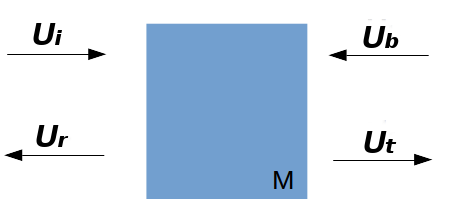
\includegraphics[width=0.6\textwidth]{images/tmm.png}
	\caption{Ilustracja podstawowego elementu w~symulacjach metodą TMM wraz z~ilustracją amplitud z~równania (\ref{eq:tmm}). Opisywanym elementem może być warstwa, granica warstw lub struktura warstwowa. }
	\label{fig:tmm-simple}
\end{SCfigure}

W przypadku analizy układu złożonego z~wielu warstw, oznaczenia ze wzoru (\ref{eq:tmm}), możemy poprzez indeks liczbowy przypisać osobno do każdej z~macierzy~$M_i$:
\begin{equation}
\begin{bmatrix}
U_i^1 \\ 
U_r^1
\end{bmatrix}
= M_1 
\begin{bmatrix}
U_t^1 \\
U_b^1
\end{bmatrix},
\label{eq:tmm-1l}
\end{equation}

\begin{equation}
	\begin{bmatrix}
	U_i^2 \\ 
	U_r^2
	\end{bmatrix}
	= M_2 
	\begin{bmatrix}
	U_t^2 \\
	U_b^2
	\end{bmatrix},
\label{eq:tmm-2l}
\end{equation}
dodając kolejne warstwy np. po lewej stronie od warstwy z~rysunku \ref{fig:tmm-simple}. Wtedy $U_i^1$ i~$U_r^1$ obliczone według wzoru \ref{eq:tmm-1l} są równe odpowiednio amplitudom $U_t^2$ i $U_b^2$ dla kolejnej warstwy we wzorze (\ref{eq:tmm-2l}). Podstawiając do wzoru \ref{eq:tmm-2l} otrzymujemy 
\begin{equation}
\begin{bmatrix}
U_i^2 \\ 
U_r^2
\end{bmatrix}
=M_2 M_1 
\begin{bmatrix}
U_t^1 \\
U_b^1
\end{bmatrix},
\label{eq:tmm-2ls}
\end{equation}
z czego wynika, że układ złożony z~$N$ warstw opisywanych macierzami przejścia $M_N$ można traktować jak jeden element opisywany za pomocą macierzy przejścia będącej iloczynem macierzy opisujących wszystkie jego elementy $M= M_i \cdot M_{i-1} ... \cdot M_1$. Podstawowymi macierzami przejścia wykorzystywanymi do obliczeń w~układach warstwowych są:
\begin{itemize}
\item Macierz przejścia odpowiadająca propagacji w~ośrodku jednorodnym 
\begin{equation}
	M_p=
	\begin{bmatrix}
	\textrm{exp}(-i k z_0) & 0 \\
	0	&\textrm{exp}(i k z_0)\\
	\end{bmatrix},
\end{equation}
gdzie $k$ jest długością wektora falowego, w~ośrodku w~którym zachodzi propagacja w~kierunku prostopadłym do granic warstw, a $z_0$ jest grubością warstwy.
\item Macierz opisująca przejście fali E-M przez granicę ośrodków
\begin{equation}
	M_i=\frac{1}{1+r}
	\begin{bmatrix}
	1 &  r \\
	 r & 1\\
	\end{bmatrix},
\end{equation}
gdzie $r$ jest amplitudowym współczynnikiem odbicia fali na opisywanej granicy ośrodków wynikającym z~równań Fresnela i~zależnym od kąta padania. Współczynnik r~może być w ogólności zespolony. Jest tak, gdy któraś z warstw ma zespoloną przenikalność elektryczną wynikającą z przewodnictwa, lub własności absorpcyjnych, a~także w~przypadku, gdy na granicy warstw zachodzi całkowite wewnętrzne odbicie i~propagacja światła przez wartwę polega na tunelowaniu optycznym.
\end{itemize}

Obliczenie współczynnika transmisji płytki płasko-równoległej wymaga więc skonstruowania macierzy opisującej taką płytkę z~trzech macierzy: 
\[
M=M_{i_1} \cdot M_p \cdot  M_{i_2}.
\]
Postępując w podobny sposób, otrzymać można macierz przejścia dla dowolnie złożonego układu warstwowego. 
